%%%%%%%%%%%%%%%%%%%%%%%%%%%%%%%%%%%%%%%%%
% Structured General Purpose Assignment
% LaTeX Template
%
% This template has been downloaded from:
% http://www.latextemplates.com
%
% Original author:
% Ted Pavlic (http://www.tedpavlic.com)
%
% Note:
% The \lipsum[#] commands throughout this template generate dummy text
% to fill the template out. These commands should all be removed when 
% writing assignment content.
%
%%%%%%%%%%%%%%%%%%%%%%%%%%%%%%%%%%%%%%%%%

\documentclass{article}

\usepackage{fancyhdr} % Required for custom headers
\usepackage{lastpage} % Required to determine the last page for the footer
\usepackage{extramarks} % Required for headers and footers
\usepackage{graphicx} % Required to insert images
\usepackage[utf8]{inputenc}

% Margins
\topmargin=-0.45in
\evensidemargin=0in
\oddsidemargin=0in
\textwidth=6.5in
\textheight=9.0in
\headsep=0.25in 

\linespread{1.1} % Line spacing



\setlength\parindent{0pt} % Removes all indentation from paragraphs

%----------------------------------------------------------------------------------------
%	DOCUMENT STRUCTURE COMMANDS
%	Skip this unless you know what you're doing
%----------------------------------------------------------------------------------------

% Header and footer for when a page split occurs within a problem environment
\newcommand{\enterProblemHeader}[1]{
\nobreak\extramarks{#1}{#1 continued on next page\ldots}\nobreak
\nobreak\extramarks{#1 (continued)}{#1 continued on next page\ldots}\nobreak
}

% Header and footer for when a page split occurs between problem environments
\newcommand{\exitProblemHeader}[1]{
\nobreak\extramarks{#1 (continued)}{#1 continued on next page\ldots}\nobreak
\nobreak\extramarks{#1}{}\nobreak
}

\setcounter{secnumdepth}{0} % Removes default section numbers
\newcounter{homeworkProblemCounter} % Creates a counter to keep track of the number of problems

%----------------------------------------------------------------------------------------
%	NAME AND CLASS SECTION
%----------------------------------------------------------------------------------------

\newcommand{\lessonNumber}[1]{Lezione\ \##1} % Assignment title
\newcommand{\lessonDate}[4]{#1,\ #2\ #3\ #4} % Due date
\newcommand{\lessonCourse}[1]{#1} % Course/class
\newcommand{\lessonTime}[1]{#1} % Class/lecture time
\newcommand{\lessonTeacher}[1]{#1} % Teacher/lecturer
\newcommand{\lessonAuthor}[1]{#1} % Your name
\begin{document}

\section{Qualit� di processo(7)}

\textit{''Dai tubi sporchi non esce acqua pulita''}\\
Voglio tecniche produttive. Quanto pi� sono produttivo tanto meno sar� reattivo. La \textbf{quality assurance} � fatta da regole, procedure e strumenti. La verifica la faccio a valle di un lavoro svolto che mi � gi� costato. Al tempo 0 ho costo 0. Voglio imparare ad essere massimamente proattivo per risparmiare risorse e fare meno fatica. E gli assi di risparmio sono assi molto importanti e rilevanti. L'intelligenza del processo sta nella sua capacit� di migliorarsi, e per migliorarsi ci si valuta, cio� ci si misura rispetto a obiettivi.

\begin{center}
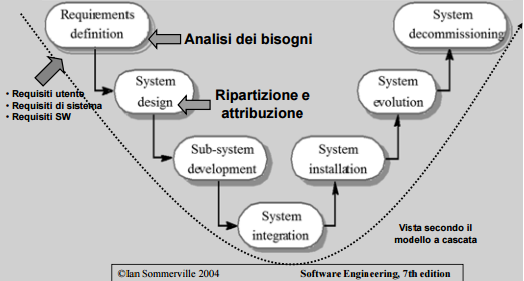
\includegraphics[width=0.75\columnwidth]{img1.png} % Example image
\end{center}

Dobbiamo crearci regole per il miglioramento e per farlo dobbiamo fare il lavoro dei processi e dei controlli. Non posso mettere il controllo su un processo non definito, quindi il primo passo � definire il processo. Ci concentreremo sulle caratteristiche che se sbagliamo ci costeranno di pi� (esempio cose che dovranno essere rifatte o che avranno conseguenze sul prodotto finale). \textbf{Norme ISO 9000-1}, � importante perch� vale come garanzia per il cliente, certifica che si lavora ad un certo livello.

\begin{center}
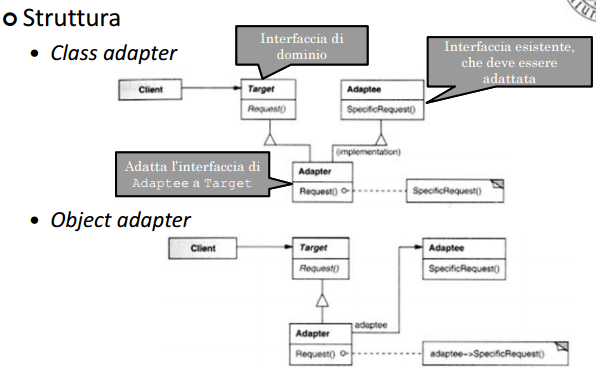
\includegraphics[width=0.75\columnwidth]{img2.png} % Example image
\end{center}


Politica di qualit� da fissare, una volta fissata posso fare un \textbf{manuale della qualit�} da cui deriva un \textbf{piano di qualit�} specifico del progetto. Le attuazioni operative del piano di qualit� includono alcune operazioni molto semplici.\\\\
\textbf{CMM}, strumento che serve per valutare come lavoriamo (\textit{Capability Maturity Model}).

\end{document}